\section{Methods}



\subsection*{React.js}

We used React.js, an innovative JavaScript library, to implement our user interface. React allows the programmer to specify different parts of the interface as {\it components}, where each component manages its own state and has its own render function. Our program has one main DrawArea component, whose state contains all the primitive shape objects, the constraints on these objects, and all the methods to draw and manipulate these objects.

The state of each object consists of where it is located in the drawing region and whether or not the shape is selected. Furthermore, each shape maintains its own render method, which is based on the aforementioned aspects of state.

Currently, we have the following shape primitives:

\begin{itemize}
\item {\bf Freehand Curves}
\item {\bf Lines}
\item {\bf Bezier Curves}
\end{itemize}

Based on these shape primitives, we created the following drawing tools:

\begin{itemize}
\item {\bf Freehand:} Simply draws a freehand curve following the cursor.
\item {\bf Polyline:} Creates lines whose endpoints are constrained to be coincident, optionally allowing the user to close the line where it started, creating a polygon.
\item {\bf Bezier:} Creates bezier curves whose endpoints are constraints to be coincident and whose control points are constrained to be collinear with their endpoints.
\item {\bf Rectangle:} Creates four lines in a rectangle where the top and bottom lines are constrained to be horizontal and the left and right lines are constrained to be vertical.
\end{itemize}

\subsection*{Geometric Constraints and Cassowary.js}

In order to design physical objects for laser cutting, we needed our program to implement geometric constraints. For example, we'd like to be able to specify two lines as parallel, or a line have fixed length. All of the constraints we wanted to implement can be represented as systems of equations. For example, if we want a point to lie on a circle of radius 1 from the origin, then we could specify the equation $x^2 + y^2 = 1$. 

The difficult part of this problem is being able to satisfy these constraints in real-time while points are changing location as the user drags them around the screen. To tackle this problem, we found Cassowary.js, a JavaScript library that implements a version of the Simplex Algorithm. The simplex algorithm is designed to solve {\it linear programming} problems, in which we must minimize a linear objective $C$, subject to certain linear constraints. For example,
\[\text{Minimize } C = x_1 + 3x_2 - 2x_4 \text{ subject to: }\]
\[x_1 + x_2 \geq 4,\]
\[x_3 - 4x_4 + x_2 = 42, \text{ and}\]
\[4x_1 + x_3 - x_2 \leq 2.\]
In the worst case, the simplex algorithm takes exponential time, but on average it takes polynomial time. Therefore, it scales very well as we add more constraints. In addition to simple linear programming, Cassowary.js also allows constraints to have a given strength, including weak, medium, strong, and required.

So, we can take our geometric constraints, and format them as constraints in a linear programming problem, where are variables are the x- and y-coordinates of certain points. For example, to make a line horizontal, we could constrain the x-coordinates of its endpoints to be equal. The issue, however, is that most geometric constraints are not naturally represented with linear equations. Our solution was to reform and approximate many geometric constraints using more than one linear equation or inequality.

\begin{itemize}
\item {\bf Fixed:} Constraints a point to stay in the same location. Implemented by setting the x-coordinate to a constant and the y-coordinate to a contsant.
\item {\bf Coincident:} Constraints two points to lie in the same location. Implemented by setting the x-coordinates to be equal and the y-coordinates to be equal.
\item {\bf Horizontal:} Constrains a line to be horizontal. Implemented by setting the x-coordinates of the two endpoints to be equal.
\item {\bf Vertical:} Constrains a line to be vertical. Implemented by setting the y-coordinates of the two endpoints to be equal.
\item {\bf Parallel:} Constrains two lines to be parallel. This constraint is more difficult to implement, as there is no way to represent it with linear equations. However, we can implement a fixed-slope constraint using linear equations. So, when this constraint is initially set, we constrain both lines to have a fixed angle, and whenever an endpoint is moved, we programmatically update the fixed-slope constraint.
\item {\bf Perpendicular:} Constrains two lines to be perpendicular. This constraint is implemented exactly the same as the parallel constraint, except for setting both lines to have the same slope, one is set to have the negative reciprocal slope of the other and is updated programmatically in a similar way.
\item {\bf Length:} Constrains a line to be a fixed length. This was the most difficult constraint to implement, as the distance equation is very nonlinear. The {\it Manhattan distance} is defined as the sum of the absolute differences between the x- and y-coordinates of two points. So, we can estimate a Euclidean distance constraint with multiple Manhattan distance constraints in the following way. If we constraint a point to be within a fixed Manhattan distance of another point, the it will lie within a diamond centered at that point. Then, using linear equations, we can transform our coordinate system by a fixed angle and set another Manhattan distance distance constraint. This constraint will have the diamond rotated by that fixed angle. Enough of these constraints will approximate a circle. However, this only constrains two points to be {\it within} a fixed distance, so we must create minimum Manhattan distance constraints in a similar way. All of these together allows us to constrain the two endpoints of a line to a fixed distance from each other. This process is illustrated in figures \ref{dist1} through \ref{dist3}.
\end{itemize}

\begin{figure}[H]
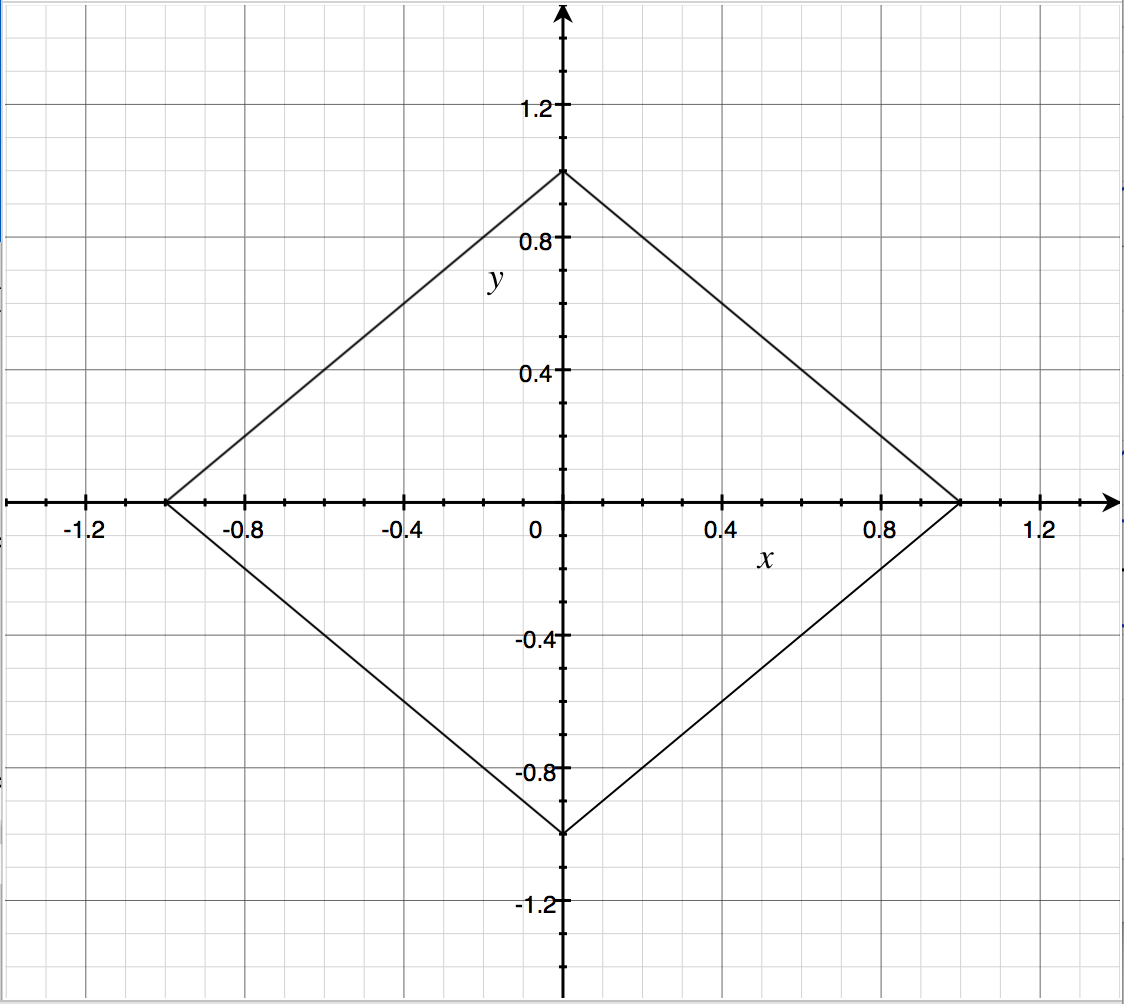
\includegraphics[scale=0.4]{dist1.png}
\caption{The region constrained by $|x| + |y| \leq 1$.}
\label{dist1}
\end{figure}

\begin{figure}[H]
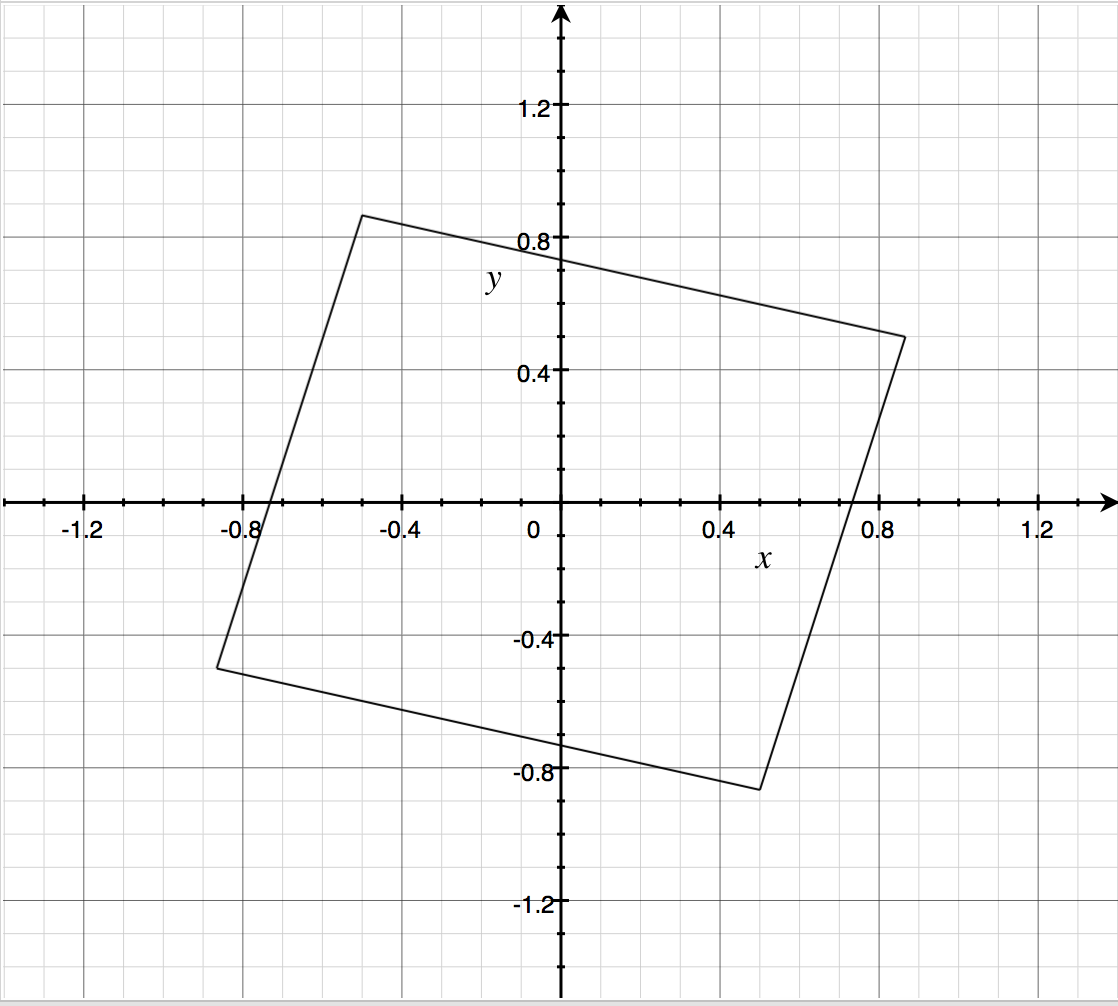
\includegraphics[scale=0.4]{dist2.png}
\caption{The region constrained by $|x'| + |y'| \leq 1$ where $x'$ and $y'$ are the coordinates of the point in the coordinate system rotated by 30$^\circ$.}
\label{dist2}
\end{figure}

\begin{figure}[H] 
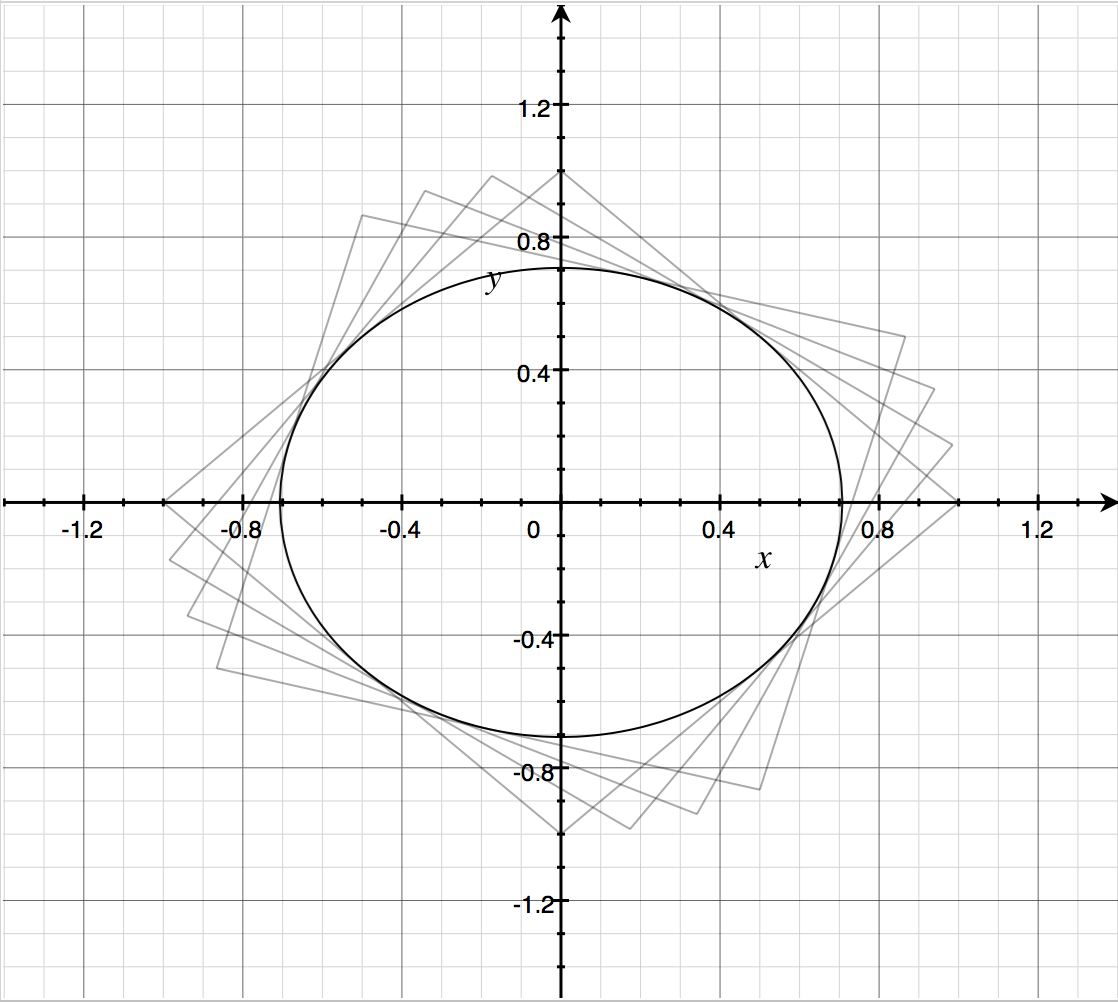
\includegraphics[scale=0.4]{dist3.png}
\caption{With enough of these regions, we approximate the region constrained to be within $\frac{\sqrt{2}}{2}$ of the origin.}
\label{dist3}
\end{figure}


\begin{figure}[H]
  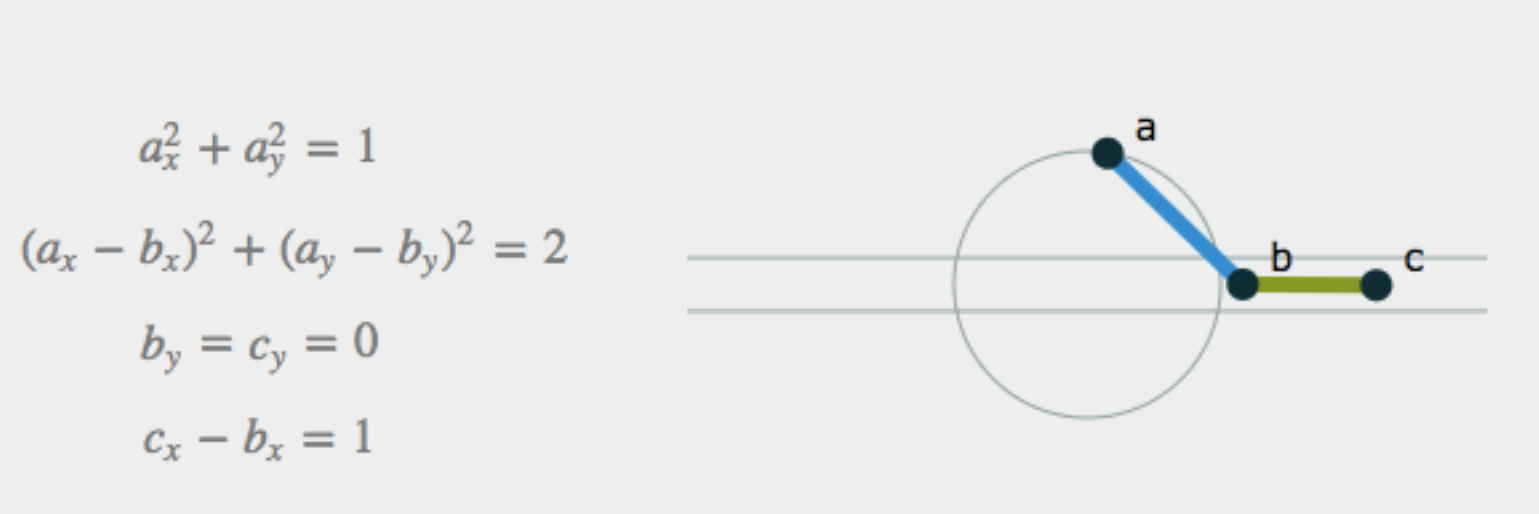
\includegraphics[width=\linewidth]{constraints.jpg}
  \caption{Parametric constraints can be represented as equations and inequalities on the values they constrain. In this figure adapted from Ref. X we constrain point a to always lie on the circle of radius 1, we fix the line with endpoints $a$ and $b$ to have length $\sqrt{2}$ using the distance equation, and we set the line with endpoints $b$ and $c$ to lie on the $x$-axis and have length 1.}
  \label{fig:constraints}
\end{figure}


\begin{comment}
This section should include the following:
\begin{itemize}
		
\item	A description of the methods you are using (which itself could have
	sub-sections). If you have created a new application, you should describe
	which tools you have used to do so and the steps of your implementation. You
	should also briefly describe each of the tools you used (e.g. Ruby on Rails,
	MongoDB, D3, etc.). If you have proposed a new algorithm to solve a problem,
	you should provide the details of your algorithm along with pseudocode. If
	your algorithm is quite complex, you should describe its running time.  

\item Description of any data you used and explanation of why you chose this
	particular data (possibly organized into sub-sections).

\item Link to a GitHub, BitBucket or other repository if relevant.

\end{itemize}
\end{comment}